\chapter{Causal analysis}
\label{ch:caus}

\section{Introduction}
\label{sec:causal_intro}

In this chapter, the application of causal inference to customer data is
explored, in the hope of shedding light on the reasons for customer churn. A
predictive experiment as conducted in the previous chapter indicates which
variables are indicative of a client about to churn, but there is no guarantee
that an intervention on any of these variables will have a positive effect. For
example, the number of contracts registered by a customer has a strong
predictive power as shown in figure
\ref{fig:var_imp_simo_diff_decrease_accuracy}. However, a hypothetical churn
retention action that would sell additional contracts will maybe fail, if
satisfied clients are more prone to buy new contracts but not dissatisfied ones.
In this case, the predictive variable  (number of contracts) and the churn have
a common cause (customer satisfaction). Manipulating the number of contracts
will therefore have no effect on churn. Different tools are needed to discover
true causal relationships between variables. In this chapter, we focus on three
types of models: causal Bayesian networks, information-theoretic filters, and
supervised causal inference. An overview of state-of-the-art methods for each of
these models is given in section \ref{sec:sota_caus}, but we describe them here
in more details.

We begin by introducing \emph{Bayesian networks}, which are graphical models
used to represent probabilistic dependencies between random variables. They are
represented by a \emph{directed acyclic graph} (DAG) where the nodes are random
variables, and a joint probability density is assigned to these variables. We
will use the terms \emph{nodes} and \emph{variable} interchangeably. In a
directed acyclic graph, a node $A$ is a parent of $B$ if there is a direct edge
from $A$ to $B$, $A$ is an ancestor of $B$ if there is a direct path from $A$ to
$B$. We can define in a similar way the notions of child, descendant,
non-descendant and spouse in a directed acyclic graph. Bayesian networks come in
a causal variant, which is defined here \parencite{guyon2007causal}.

\begin{definition}[Causal Bayesian network]

Let $\bm X$ be a set of random variables and $P$ a joint
probability density over $\bm X$. Let $\Gamma$ be a DAG in which the vertices
are $\bm X$. It is required that
\begin{enumerate}[(i)]
    \item for every edge from a node $X\in\bm X$ to a node $Y\in\bm X$, $X$ is a
    direct cause of $Y$, and
    \item for every node $X\in\bm X$, $X$ is probabilistically independent of
    all its non-descendants, given its parents.
\end{enumerate}
The first condition is required for a Bayesian network to be causal, and the
second condition is called the Markov condition. The tuple $(\bm X, P, \Gamma)$
is a causal Bayesian network iff both conditions are satisfied.

\end{definition}

We denote independence between two variables $A$ and $B$ according to the
probability density $P$ as $A\perp_P B$. Similarly, the conditional independence
between two variables $A$ and $B$ given a set of variables $\bm C$ is written
$A\perp_P B|\bm C$. Using the notion of \emph{d-separation} as introduced by
Pearl (\emph{e.g.} in \cite{pearl2002causality}), we define the conditional
independence between two variables $A$ and $B$ entailed by the Markov condition
on a DAG $\Gamma$ as $A\perp_\Gamma B|\bm C$.

The condition of \emph{faithfulness} is often set onto a causal Bayesian
network:

\begin{definition}[Faithfulness]
\label{def:faith}

A DAG $\Gamma$ is \emph{faithful} to a joint probability density $P$ iff every
dependency entailed by the Markov condition on $\Gamma$ is also
entailed by $P$. That is,

\begin{equation}
\forall X, Y\in\bm X,\forall \bm Z\subset\bm X,\quad
X\not\perp_\Gamma Y|\bm Z\Rightarrow X\not\perp_P Y|\bm Z.
\end{equation}

\end{definition}

Both the Markov conditions and the faithfulness conditions ensure that a given
graph and a given probability density represent accurately the same set of
dependencies and independencies. When both conditions are met, we write
(in)dependence relations without specifying whether it is entailed by $P$ or
$\Gamma$. The faithfulness condition, in particular, ensures that the influence
of a cause onto an effect by multiple causal routes does not cancel itself out.
To demonstrate a violation of this assumption, assumes that a gene codes both
for the production of a particular protein and for the suppression of another
gene that codes this protein as well. In this case, when the first gene is
removed, the protein is still produced by the other gene, and therefore the
presence of the first gene seems to be independent of the production of the
protein. The probability density $P$ postulates the independence between the two
variables, whereas the causal structure of the problem indicates a causal
link\parencite{hitchcock1997probabilistic}.

Another important concept in Bayesian networks is the notion of \emph{Markov
blanket} of a variable. Informally, this is a set of variables that shields a
given target variable from the influence of the rest of the network. This notion
is useful, for example, in feature selection for machine learning. The Markov
blanket of a target variable is a subset that brings the maximum information
about the target, among all possible sets of variables. Adding any other
variable will bring some information that is already contained in other members,
or in the interaction thereof, of the Markov blanket.

\begin{definition}[Markov blanket]

For a set of random variables $\bm X$, a subset $\bm M\subset\bm X$ and a
variable $Y\in\bm X$, $\bm M$ is the Markov blanket of $Y$ iff for any subset
$\bm V\subset\bm X$, $Y$ is conditionnally independent of $\bm V\setminus \bm M$
given $\bm M$.

\end{definition}

In our case, where causal Bayesian networks are represented by a directed
acyclic graph, and where both the Markov and the faithfulness
conditions are met, the Markov blanket of a variable is unique and consists of
its direct causes, its direct effects, and the direct causes of its direct1235711
effects. An example is given on figure \ref{fig:markov_blanket}.

\begin{figure}
    \centering
    \begin{tikzpicture}
        \tikzset{every node/.style={circle, thick},
                >={Stealth[black]},
                every edge/.style={draw=black,very thick}}

        \node[fill=lightorange, draw, minimum size=2.4em] (1) at (0, 0) {$Y$};
        \node[fill=lightblue, draw] (2) at (-1.5, 1.5) {$C_1$};
        \node[fill=lightblue, draw] (3) at (1.5, 1.5) {$C_2$};
        \node[fill=lightblue, draw] (4) at (-1.5, -1.5) {$E_1$};
        \node[fill=lightblue, draw] (5) at (1.5, -1.5) {$E_2$};
        \node[fill=lightblue, draw] (6) at (3, 0) {$S_1$};
        \node[draw] (7) at (-3, 3) {$A_1$};
        \node[draw] (8) at (-3, 0) {$D_1$};
        \node[draw] (9) at (3, 3) {$A_2$};
        \node[draw] (10) at (4.5, 1.5) {$Z_1$};

        \path [->] (2) edge node {} (1);
        \path [->] (3) edge node {} (1);
        \path [->] (1) edge node {} (4);
        \path [->] (1) edge node {} (5);
        \path [->] (6) edge node {} (5);
        \path [->] (7) edge node {} (2);
        \path [->] (4) edge node {} (8);
        \path [->] (9) edge node {} (3);
        \path [->] (10) edge node {} (6);

    \end{tikzpicture}
    \caption{A causal Bayesian network, with the Markov blanket of $Y$
    highlighted in blue.}
    \label{fig:markov_blanket}
\end{figure}

These definitions lay the theoretical background for graphical causal models,
but methods for inference from observational data still need to be derived. The
methods used in this experiment are described in section
\ref{sec:causal_experiments}. A common requirement of some of these methods is
an accurate test of statistical independence between two variables in $\bm X$.
Many statistical independence tests exist, but in our case, we need an estimator
that is able to handle a mix of categorical and continuous variables. We use the
\emph{mutual information}, which is an information-theoretic measure of
statistical dependency. It is more general than the Pearson or the Spearman
correlation coefficient, as it encompasses any type of dependency, and not only
linear or monotonic relationships. Also, it is defined for any two random
variables, regardless of their type or domain. In the case of two discrete
variables $X$ and $Y$ taking values respectively in $\mathcal X$ and $\mathcal
Y$, with a joint probability distribution $P(X, Y)$ and marginal probability
distributions $P(X)$ and $P(Y)$, the mutual information between $X$ and  $Y$ is
defined as \parencite{cover2012elements}

\begin{align}
    I(X, Y) &= \sum_{x\in\mathcal X}\sum_{y\in\mathcal Y}
    P(x, y) \log\left(\frac{P(x, y)}{P(x)P(y)}\right)\label{eq:mi_discrete}\\
    &= H(X) - H(X|Y)\\
    &= H(Y) - H(Y|X)\\
    &=H(X) + H(Y) - H(X, Y)
\end{align}

where $H(X)$ is the entropy of $X$ and $H(X|Y)$ is the conditional entropy of
$X$ given $Y$\parencite{shannon1948mathematical}. The two last equalities
indicate that the mutual information is a symmetric, positive quantity, and
that it can be viewed as the reduction in uncertainty that a variable brings
about the other. A schematic view of these formulae is given in figure
\ref{fig:mi_schematic}. In the case of two continuous variables, an analogous
definition exist \parencite{kolmogorov1956shannon}

\begin{figure}
    \centering
    \begin{tikzpicture}
        \fill[lightblue, opacity = 0.5] (-1,0) circle (1.8);
        \fill[lightorange, opacity = 0.5] (1,0) circle (1.8);
        \draw (-1,0) circle (1.8) node [left] {$H(X|Y)$};
        \draw (1,0) circle (1.8) node [right] {$H(Y|X)$};
        \node at (0,0) {$I(X, Y)$};
        \node at (-3.5,0) {$H(X)$};
        \node at (3.5,0) {$H(Y)$};
        \node at (0,2.2) {$H(X, Y)$};
    \end{tikzpicture}
    \caption{Schematic representation of the relationship between entropy,
    conditional entropy, joint entropy, and mutual information of two discrete
    random variables.}
    \label{fig:mi_schematic}
\end{figure}

\begin{align}
    I(X, Y) &= \int_\mathcal X\int_\mathcal Y
    P(x, y) \log\left(\frac{P(x, y)}{P(x)P(y)}\right)dx\,dy\\
    &= h(X) - h(X|Y)\\
    &= h(Y) - h(Y|X)\\
    &= h(X) + h(Y) - h(X, Y)
\end{align}

where $h(X)$ is the differential entropy of $X$ and $h(X|Y)$ is the conditional
differential entropy of $X$ given $Y$. In the case of two normally distributed
variables, we have

\begin{equation}
    \label{eq:mi_gaussian}
    I(X,Y)=-\frac{1}{2}\log(1-\rho^2)
\end{equation}

where $\rho$ is the Pearson correlation coefficient between $X$ and $Y$. Even
though the assumption of normal distribution does not hold in general, empirical
results show that it is still a decent estimator for non-linear dependencies
\parencite{olsen2008impact}. Finally, the mutual information between a continuous
variable $X$ and a discrete variable $Y$ taking values in a finite set $\mathcal
Y$ can be computed as

\begin{equation}
I(X, Y)=h(X) - h(X|Y)=h(X)-\sum_{y\in\mathcal Y}h(X|Y=y)P(Y=y)\label{eq:mi_mixed}
\end{equation}

which means that the mutual information in the mixed case can be computed with
an estimator of the differential entropy of a continuous variable. Following the
discretization method described in \parencite{olsen2008impact}, let $N$ be the
number of values sampled iid from $X$. We divide the domain $\mathcal X$ of $X$
into $k$ bins of equal size $\Delta$, and we write $\text{nb}(i)$ the number of
samples present in the $i$th bin, $\forall i\in\{1,\dots,k\}$. The differential
entropy of $X$ is estimated with the \emph{Miller-Madow estimator}

\begin{equation}
    \label{eq:mle_ent}
    \hat h(X) = \sum_{i=1}^k
    \frac{\text{nb}(i)}{N}\log\left(\frac{\text{nb}(i)}{N}\right) + \log\Delta +
    \frac{k-1}{2N}
\end{equation}

It follows that we can compute the mutual information in all possible
configurations of variable types:
\begin{enumerate}[(i)]
    \item Between two discrete variables, using equation \ref{eq:mi_discrete}
    \item Between a continuous variable $X$ and a discrete variable $Y$ with
    equation \ref{eq:mi_mixed} and the differential entropy estimator of
    equation \ref{eq:mle_ent}
    \item Between two continuous variables assuming normal distributions with
    equation \ref{eq:mi_gaussian}
\end{enumerate}

The mutual information can be generalized for any $n$ variables, and is then
named $n$-way \emph{interaction} or \emph{co-information}
\parencite{bell2003co}. A general formula exists, but we are only interested in
the case $n=3$ since it is connected with causal configurations composed of
three variables. In this case, the 3-way interaction (that we simply name
interaction) between three random variables $X_1$, $X_2$, and $Y$ is defined in
\parencite{mcgill1954multivariate} as

\begin{equation}
    \label{eq:int_cond}
    I(X_1, X_2, Y) = I(X_1, X_2) - I(X_1, X_2 | Y)
\end{equation}

where, in the case of a discrete $Y$ taking values in a finite set $\mathcal
Y$, $I(X_1, X_2 | Y)$ can be computed as

\begin{equation}
    \label{eq:int_cond_sum}
    I(X_1, X_2 | Y) = \sum_{y\in\mathcal Y}P(Y=y)I(X_1, X_2 | Y = y)
\end{equation}

A more general definition of conditional mutual information is given in
\parencite{cover2012elements}. But since we consider a classification problem
with $\mathcal Y = \{0, 1\}$, this restricted definition is sufficient for our
purposes.

\section{Scope}

In this chapter, the same dataset as in the predictive modeling chapter is used.
We restrict ourselves to SIM only contracts since it is supposed that the causes
of churn are at least partially different between loyalty and SIM only
contracts. All 5 months of data are used. In order to decrease computation time,
only the first 30 variables in the ranking of the random forest trained in
chapter \ref{ch:churn} are used. Depending on the algorithm being used, a random
subsampling has been applied, also to reach decent computation times. In all
cases, the positive class (churners) is untouched, and a random subset of the
negative class is sampled so that the class ratio is even.

\section{Prior knowledge on churn}
\label{sec:causal_prior}

Bayesian reasoning indicates that we should always take into account our prior
knowledge on a problem when considering the outcome of an experiment designed to
test some hypotheses on this problem. An unlikely theory according to our priors
needs strong evidence to be proven true. Ideally, we should assign a probability
(in the Bayesian sense, that is, a degree of belief) to every theory, and
calculate the probability of the experiment results according to each theory. We
will obviously not conduct this procedure formally in the context of this study,
but the Bayesian methodology is nonetheless useful to keep in mind when
interpreting the results of the causal inference experiments. This section
describes the prior knowledge we have on the causes of churn. It is the result
of discussions and interviews with the data science and business intelligence
teams at Orange Belgium. This prior knowledge is highly valuable, since it
incorporates years of experience in churn prevention and customer relationship
in general. We summarize the main causes of churn in four different settings.

\paragraph{Bill shock} This setting has been already evoked multiple times in
chapter \ref{ch:churn}. It occurs when a customer has an unusually large
service usage, which results in an important out of bundle amount (i.e. the
client is charged much more than usual). This triggers a reaction from the
customer inducing an increased risk of churn. This scenario is well understood
and verified in practice. It is believed to be the most important cause of
churn.

\paragraph{Customer dissatisfaction} Multiple factors influence the customer
satisfaction, including the quality of service and the network quality. A
customer having numerous cuts of network connection during phone calls, or
unable to use properly Orange online services, will be more likely to seek
better alternatives elsewhere.

\paragraph{Wrong positioning} Each customer has different service usage habits.
Some people make a few minutes of phone calls per month, whereas this can be
counted in hour for others. This is why multiple tariff plan are proposed by the
service provider. However, choosing the right tariff plan is sometimes
difficult. On the one hand, if not enough call time is provisioned, an out of
bundle amount is likely to be charged at the end of the month. On the other
hand, an expensive tariff plan results in a high fixed cost for the customer.
When the tariff plan of the customer does not correspond to her needs, we say
that the customer is wrongly positioned. A wrong positionnement results in most
cases to a higher bill that expected, and is a significant cause of churn.

\paragraph{Churn due to a move} It is common to choose a product bundle from a
telecommunication company comprising a subscription for mobile phone, landline
phone, television and internet connection. In this case, the subscription is
tied to the particular place of domicile of the customer. When the client moves
to another place, it is quite common to also change to another telecommunication
provider. This is therefore a significant cause of churn, albeit of a different
nature from the other settings previously exposed.


\paragraph{} These different settings are described informally, and their
translation to the formal definitions of causality presented in section
\ref{sec:causal_intro} is not straightforward. This touches upon philosophical
debates on the definition of causality, which are well beyond the scope of this
thesis. More practically, we wish to find a mapping between the events believed
to be causes of churn, and specific instanciations of measurable random
variables. In the case of the first setting, we can reasonably assume that
variables measuring the out of bundle amount of the customer is a faithful proxy
for bill shock.  Similarly, the customer satisfaction can be estimated using,
for example, the number of network cuts during phone calls, or the number of
calls to the customer service. The wrong positioning can also be numerically
estimated, given the tariff plan of the client and its average service usage.
The last setting, churn due to a move, is much more difficult to estimate, as it
is not directly related to the interaction between the client and the
telecommunication services.

In the dataset available for this study, the only measured variables that
translate to potential causes of churn are the ouf of bundle, the tariff plan
and the service usage (phone calls, messages, mobile data). We have no measure
for network quality, customer satisfaction, or propensity to move in the near
future. Also, the wrong positioning is not explicitly encoded and has to be
inferred by the causal inference model from the average service usage and the
current tariff plan.

\section{Experiments}
\label{sec:causal_experiments}

The overall scheme of this experiment consists of running several causal
inference techniques, which give different types of results in various forms,
and extract a general consensus, if any, in the light of the different
assumptions each model put on the data. Indeed, all causal inference methods are
based on different assumptions, and the ability of a given method to infer
causal patterns from observational data lies upon these assumptions.

More specifically, we use 5 different causal inference algorithms:
\noprelistbreak
\begin{itemize}
    \item PC
	\item Grow-shrink (GS)
	\item Incremental Association Markov Blanket (IAMB)
	\item Minimum interaction maximum relevance (mIMR)
	\item D2C
\end{itemize}

For the first three methods, we use the R package \emph{bnlearn}
\parencite{scutari2009learning} for independence tests using mutual information
and asymptotic $\chi^2$ test \parencite{good2013permutation}. For mIMR and D2C,
we use the R package \emph{D2C} \parencite{bontempi2015dependency}, along with
another implementation of mIMR using the mutual information estimator given in
section \ref{sec:causal_intro}. The sample size used in the experiment is given
after the description of each algorithm. In all cases, a false positive rate of
0.05 is chosen for statistical tests of independence.

\subsection{PC}

\paragraph{Description} The PC algorithm \parencite{spirtes1991algorithm} returns
the set of directed acyclic graphs that are faithful to a given probability
distribution. It is based on independence tests between two variables,
conditioned on a set of other variables. It uses the notion of d-separation to
eliminate or find the direction of putative causal links. The PC algorithm is
given in algorithm \ref{alg:pc}, where $\textbf{Adjacencies}(X)$ is the current
set of nodes that are adjacent to $X$ in $\Gamma$. Therefore, it evolves as
$\Gamma$ is modified in the algorithm. The idea underlying PC is to A) start
with a full graph, B) remove edges using independence tests with conditioning
sets of increasing size, C) orient colliders using the d-separation property,
and D) find remaining orientations using two more rules. The assumptions
underlying this algorithm are

\begin{enumerate}[(i)]
    \item There is no unmeasured confounder
    \item The statistical tests are correct
    \item The causal relationships between variables are the same for all samples
    \item There exists a DAG $\Gamma$ representing the causal structure that is
    faithful to the underlying joint probability density $P$ (definition
    \ref{def:faith})
\end{enumerate}

If these assumptions hold, then the result of the algorithm is a set of DAGs
that are all faithful to the density probability $P$. The assumption (iii) is
reasonable in our case, but the three others less so.

\begin{algorithm}
    \caption{The PC algorithm}
    \label{alg:pc}
    \begin{algorithmic}
        \State A) Let $\Gamma$ be a complete undirected graph on the set of
        vertices $\bm X$.

        \State B) $n\gets 0$
        \Repeat
            \Repeat
                \State Select a pair of vertices $X$ and $Y$ such that
                \State $\quad\bullet\;X$ and $Y$ are adjacent
                \State $\quad\bullet\;$ there exists a set $\bm
                Z\subseteq\textbf{Adjacencies}(X)\setminus \{Y\}$ that has $n$
                elements
                \State $\quad\bullet\;$ $X\perp Y|\bm Z$.
                \State Remove the edge $X \text{---} Y$ from $\Gamma$
                \State Add $\bm Z$ to $\textbf{Sepset}(X, Y)$ and to $\textbf{Sepset}(Y, X)$
            \Until {no $X$, $Y$ pairs satisfying above conditions can be found}
            \State $n\gets n+1$
        \Until {for each pair $X$ and $Y$, $|\textbf{Adjacencies}(X)\setminus \{Y\}|<n$}

        \State C) For all triplets $X \text{---} Y \text{---} Z$ where there is
        no edge between $X$ and $Z$, orient it as $X\rightarrow Y \leftarrow Z$
        if $Y$ is not in $\textbf{Sepset}(X, Z)$

        \State D)
        \Repeat
            \State Orient all $X\rightarrow Y\text{---} Z$ as $X\rightarrow Y
            \leftarrow Z$
            \State Orient all $X\text{---}Y$ as $X\rightarrow Y$ if there is
            a directed path from $X$ to $Y$
        \Until{no more edges can be oriented}
    \end{algorithmic}
\end{algorithm}

\paragraph{Experimental setting} The PC algorithm is slow when the number of
samples is large since the whole Bayesian network is inferred. Therefore, we
restrict the dataset to 10,000 samples. The implementation given in the package
\emph{bnlearn} is used. The results are given under the form of a directed
acyclic graph.

\subsection{Grow-Shrink}

\paragraph{Description} The GS algorithm \parencite{margaritis2000bayesian} is a
Markov Blanket discovery algorithm efficient even for a large number of
variables. It is based on an estimator that returns a numerical value for the
statistical dependency between two variables, potentially conditioned on a set
of other variables. In our case, we use the mutual information. Consider a
target variable $Y$ and a set of predictor variables $\bm X$. The GS algorithm
constructs the Markov blanket of $Y$, denoted $\MB(Y)$, in three phases
performed in sequence:

\begin{enumerate}[A)]
    \item All variables $X\in\bm X$ are ordered in decreasing order according to
    $I(X, Y)$
    \item Each variable $X\in\bm X$ is added to $\MB(Y)$ iff it is
    conditionally dependent on $Y$, given $\MB(Y)$. That is, iff $I(X,
    Y|\MB(Y)) > 0$.
    \item Each variable $X\in\MB(Y)$ is removed from $\MB(Y)$
    iff it is conditionally independent of the rest of $\MB(Y)$. That
    is, iff $I(X, Y|\MB(Y)\setminus\{X\}) = 0$.
\end{enumerate}

The phase A) is a heuristic to speed up the search, however
\textcite{tsamardinos2003algorithms} pointed out that this delays the inclusion
of spouses, since those have small unconditional relevance to $Y$. Therefore,
more false positives are included before spouses get into $\MB(Y)$.

\paragraph{Experimental setting} The entire set of positive samples is used,
along with a subset of the same size of negative samples. This amounts to a
total of 240,168 samples. The GS algorithm has been implemented using the
independence test in the package \emph{bnlearn}. The results are given as a
list of members of the Markov blanket.


\subsection{Incremental Association Markov Blanket}

\paragraph{Description} The IAMB algorithm \parencite{tsamardinos2003algorithms}
is essentially similar to the GS algorithm, but does not include the sorting
heuristic as a first phase:

\begin{enumerate}[A)]
    \item The variable $X\in\bm X$ maximizing $I(X, Y|\MB(Y))$ is added
    to $\MB(Y)$, repeatedly until all remaining variables are
    independent of $Y$ given $\MB(Y)$.
    \item Each variable $X\in\MB(Y)$ is removed from $\MB(Y)$
    iff it is conditionally independent of the rest of $\MB(Y)$. That
    is, iff $I(X, Y|\MB(Y)\setminus\{X\}) = 0$.
\end{enumerate}

\paragraph{Experimental setting} The experimental setting is the same as for
the GS algorithm.

\subsection{Minimum Interaction Maximum Relevance}

\paragraph{Description} The mIMR filter \parencite{bontempi2010causal} is a
feature selection algorithm that has similarities with the mRMR algorithm
\parencite{peng2005feature}. By using the interaction instead of the redundancy
between the candidate variable and the set of selected variables, causes and
spouses of the target are favored. In order to select only causes, spouses are
eliminated beforehand on the basis of their null unconditional mutual
information with the target. More formally, the main objective of feature
selection is to find a subset $\bm X^*$ of a set of variables $\bm X$ that
maximizes the mutual information with the target $Y$:

\begin{equation}
\bm X^*=\argmax_{\bm X_S\subseteq \bm X} I(\bm X_S,Y)
\end{equation}

Evaluating all possible subsets $\bm X_S$ is computationally infeasible, the
forward selection scheme is therefore adopted. It consists in repetitively
selecting the variable $X_{d+1}^*$ that bring the most improvement given the set
$\bm X_S$ containing the $d$ variables already selected, until a fixed number
$v$ of variables is attained. The improvement is determined in a way that favors
direct causes of $Y$. Consider the interaction equation \ref{eq:int_cond}. The
interaction $I(X_1, X_2, Y)$ can be viewed as the reduction in statistical
dependency between $X_1$ and $X_2$ brought by the knowledge of $Y$. On the one
hand, a positive interaction occurs in 4 types of causal patterns, shown in
figures \ref{fig:chain}, \subref{fig:common_cause}, \subref{fig:brotherhood} and
\subref{fig:grandparent}. On the other hand, a negative interaction occurs only
in the common cause configuration (figure \ref{fig:common_cause}) and the spouse
configuration (figure \ref{fig:spouse}). Furthermore, one can differentiate
between common causes and spouses by noticing that a spouse of the target has
null unconditional relevance with the target (a spouse is relevant only when the
common effect is known). In practice, a statistical test is used to determine
the set of variables having non-null mutual information with the target, written
$\bm X_+$. This leads to the update criterion of mIMR that is a linear
combination of relevance and interaction:

\begin{equation}
    X_{d+1}^* = \argmax_{X_k\in\bm X_+ \setminus \bm X_S}
    \left[ I(X_k,Y) - I(\bm X_S, X_k, Y)\right].
\end{equation}

\begin{figure}
    \centering
    \begin{subfigure}[b]{0.3\linewidth}
        \begin{tikzpicture}
            \tikzset{every node/.style={circle, thick},
                    >={Stealth[black]},
                    every edge/.style={draw=black,very thick}}
            \node[draw, minimum size=2.4em] (1) at (0, 0) {$Y$};
            \node[draw] (2) at (-1.5, 1.5) {$X_1$};
            \node[draw] (3) at (1.5, 1.5) {$X_2$};
            \path [->] (2) edge node {} (1);
            \path [->] (3) edge node {} (1);
        \end{tikzpicture}
        \caption{Common effect}
        \label{fig:common_effect}
    \end{subfigure}
    ~
    \begin{subfigure}[b]{0.3\linewidth}
        \begin{tikzpicture}
            \tikzset{every node/.style={circle, thick},
                    >={Stealth[black]},
                    every edge/.style={draw=black,very thick}}
            \node[draw] (1) at (0, 0) {$X_1$};
            \node[draw] (2) at (-1.5, 1.5) {$X_2$};
            \node[draw, minimum size=2.4em] (3) at (1.5, 1.5) {$Y$};
            \path [->] (2) edge node {} (1);
            \path [->] (3) edge node {} (1);
        \end{tikzpicture}
        \caption{Spouse}
        \label{fig:spouse}
    \end{subfigure}
    ~
    \begin{subfigure}[b]{0.3\linewidth}
        \begin{tikzpicture}
            \tikzset{every node/.style={circle, thick},
                    >={Stealth[black]},
                    every edge/.style={draw=black,very thick}}
            \node[draw, minimum size=2.4em] (1) at (0, 0) {$Y$};
            \node[draw] (2) at (-2, 0) {$X_1$};
            \node[draw] (3) at (2, 0) {$X_2$};
            \path [->] (2) edge node {} (1);
            \path [->] (1) edge node {} (3);
        \end{tikzpicture}
        \caption{Chain}
        \label{fig:chain}
    \end{subfigure}
    ~
    \begin{subfigure}[b]{0.3\linewidth}
        \begin{tikzpicture}
            \tikzset{every node/.style={circle, thick},
                    >={Stealth[black]},
                    every edge/.style={draw=black,very thick}}
            \node[draw, minimum size=2.4em] (1) at (0, 0) {$Y$};
            \node[draw] (2) at (-1.5, -1.5) {$X_1$};
            \node[draw] (3) at (1.5, -1.5) {$X_2$};
            \path [->] (1) edge node {} (2);
            \path [->] (1) edge node {} (3);
        \end{tikzpicture}
        \caption{Common cause}
        \label{fig:common_cause}
    \end{subfigure}
    ~
    \begin{subfigure}[b]{0.3\linewidth}
        \begin{tikzpicture}
            \tikzset{every node/.style={circle, thick},
                    >={Stealth[black]},
                    every edge/.style={draw=black,very thick}}
            \node[draw] (1) at (0, 0) {$X_1$};
            \node[draw, minimum size=2.4em] (2) at (-1.5, -1.5) {$Y$};
            \node[draw] (3) at (1.5, -1.5) {$X_2$};
            \path [->] (1) edge node {} (2);
            \path [->] (1) edge node {} (3);
        \end{tikzpicture}
        \caption{Brotherhood}
        \label{fig:brotherhood}
    \end{subfigure}
    ~
    \begin{subfigure}[b]{0.3\linewidth}
        \begin{tikzpicture}
            \tikzset{every node/.style={circle, thick},
                    >={Stealth[black]},
                    every edge/.style={draw=black,very thick}}
            \node[draw, minimum size=2.4em] (1) at (0, 0) {$X_1$};
            \node[draw] (2) at (-2, 0) {$X_2$};
            \node[draw, minimum size=2.4em] (3) at (2, 0) {$Y$};
            \path [->] (2) edge node {} (1);
            \path [->] (1) edge node {} (3);
        \end{tikzpicture}
        \caption{Grandparent}
        \label{fig:grandparent}
    \end{subfigure}

    \caption{Possible causal patterns between two variables $X_1$ and $X_2$ and
    a target variable $Y$ having non-null interaction.}
    \label{fig:markov_blanket}
\end{figure}

Using the approximation

\begin{equation}
    I(\bm X_S, X_k, Y) \approx \frac{1}{d}\sum_{X_i\in\bm X_S} I(X_i, X_k, Y),
\end{equation}

the forward step can be written as

\begin{align}
    X_{d+1}^* &= \argmax_{X_k\in\bm X_+ \setminus \bm X_S}
    \left[I(X_k,Y) - \frac{1}{d}\sum_{X_i\in\bm X_S} I(X_i, X_k, Y)\right]\\
    &= \argmax_{X_k\in\bm X_+ \setminus \bm X_S}
    \left[I(X_k,Y) - \frac{1}{d}\sum_{X_i\in\bm X_S}
    \left(I(X_i,X_k)-I(X_i, X_k,|Y)\right)\right]\label{eq:mimr_int}\\
    &= \argmax_{X_k\in\bm X_+ \setminus \bm X_S}
    \left[I(X_k,Y) + \frac{1}{d}\sum_{X_i\in\bm X_S} \sum_{y\in\mathcal Y}
    P(Y = y)\left(I(X_i, X_k,|Y=y)-I(X_i,X_k)\right)\right]\label{eq:mimr_final}
\end{align}

where equation \ref{eq:mimr_int} is derived using equation \ref{eq:int_cond} and
similarly \ref{eq:mimr_final} is derived from \ref{eq:int_cond_sum}. The first two variables are selected as

\begin{equation}
    X_1^*, X_2^* = \argmax_{X_i, X_k\in\bm X_+}I([X_i,X_k],Y).
\end{equation}

The mIMR filter is based on some underlying estimator of mutual information
between two variables, and a statistical test of independence for selecting the
set of unconditionally relevant variables.

\paragraph{Experimental setting} In this experiment, two implementations are
used:
\noprelistbreak
\begin{itemize}
    \item One using the mutual information estimator described in section
    \ref{sec:causal_intro} and the test of independence in the package
    \emph{bnlearn}.
    \item One assuming normally-distributed continuous variables, allowing to
    compute the mutual information (with equation \ref{eq:mi_gaussian}) and to
    test for independence using the Pearson correlation coefficient. Discrete
    variables are converted to numerical values using one-hot encoding.
\end{itemize}

The drawback of the first method is that the mutual information estimator is
ad-hoc: it assumes a monotonic relationship between two continuous variables
but uses a histogram-based entropy estimator in the mixed case. This may lead to
inconsistencies in the measure of mutual information. On the other hand, the
second method sets the linear assumption on all variables, even on one-hot
encoded categorical variables. For the first implementation, the dataset is
restricted to 10,000 samples, due to the computational cost of the entropy
estimator. In the second implementation, 100,000 samples are used. The results
are provided as a list of the first 15 selected variables, accompanied with the
gain provided by each variable at each iteration of the algorithm.

\subsection{D2C}

\paragraph{Description} The first three causal inference algorithms used in this
section are solely based on statistical independence tests, and therefore are
unable to differentiate between indistinguishable causal patterns, such as the
two variables configuration or the fully-connected three variables
configuration. Since the probability density $P$ is reduced to a set of
(in)dependence relations, any fully connected graph is faithful to $P$ in these
two cases. Asymmetrical patterns exist however in the joint probability density
of a cause and its effect, as demonstrated by the results of the Kaggle
competition Cause-effect pairs
(\url{https://www.kaggle.com/c/cause-effect-pairs}). The D2C algorithm
\parencite{bontempi2015dependency} is based on the asymmetry of descriptor
extracted from the Markov blanket of two causally linked variables. Consider two
random variables $X_1$ and $X_2$ such that $X_1$ is a cause of $X_2$, and their
respective Markov blanket $\MB(X_1)$ and $\MB(X_2)$. This setting is pictured in
figure \ref{fig:d2c_mb}. We consider only one cause, effect and spouse per
Markov blanket for the sake of the presentation, but the principles generalize
obviously to any Markov blanket. Even though we cannot distinguish between
causes, effects and spouses among $\MB(X_1)$ and $\MB(X_2)$, we can derive
several inequalities using d-separation. Consider the variables $M_1$ and $M_2$,
which are members of respectively  $\MB(X_1)$ and $\MB(X_2)$, but whose relation
to $X_1$ and $X_2$ is unknown (that is, $M_1$ is either $C_1$, $E_1$ or $S_1$).
We have

\begin{equation}
\label{eq:d2c_ineq}
\begin{cases}
    I(X_1, M_2 | X_2) > I(X_2, M_1 | X_1)\quad\text{if }M_2 = C_2 \\
    I(X_1, M_2 | X_2) = I(X_2, M_1 | X_1)\quad\text{otherwise,}
\end{cases}
\end{equation}

since the only collider configuration between one of $X_1$ and $X_2$ and a
member of the Markov blanket of the other variable is $X_1\rightarrow
X_2\leftarrow C_1$. By computing a population of descriptors

\begin{align}
    D(1, 2)&=\{I(X_1, M_2 | X_2)|\;\forall M_2\in\MB(X_2)\}\\
    D(2, 1)&=\{I(X_2, M_1 | X_1)|\;\forall M_1\in\MB(X_1),\},
\end{align}

equation \ref{eq:d2c_ineq} indicates that the distribution of $D(1, 2)$ differs
from $D(2, 1)$. Other similar inequalities are used to compute 2 other
population of descriptors. The rank of each $M_1$ in $\MB(X_2)$ is also
computed, along with the rank of each $M_2$ in $\MB(X_1)$. The quartiles of the
population of these various descriptors are computed, along with the
mutual information between $X_1$ and $X_2$, and the mutual information
conditioned on $\MB(X_1)$ or $\MB(X_2)$. All these quantities are then used as
features on a machine learning algorithm, whose task is to predict the
probability of a causal link between $X_1$ and $X_2$. The default implementation
of D2C uses a random forest classifier.

\begin{figure}
    \centering
    \begin{tikzpicture}
        \tikzset{every node/.style={circle, thick},
                >={Stealth[black]},
                every edge/.style={draw=black,very thick}}

        \node[draw, minimum size=2.4em] (1) at (0, 0) {$X_1$};
        \node[fill=lightorange, draw] (2) at (1.5, 1.5) {$C_1$};
        \node[fill=lightorange, draw] (3) at (-1.5, -1.5) {$E_1$};
        \node[fill=lightorange, draw] (4) at (-3, 0) {$S_1$};
        \node[draw] (5) at (3, -3) {$X_2$};
        \node[fill=lightblue, draw] (6) at (4.5, -1.5) {$C_2$};
        \node[fill=lightblue, draw] (7) at (1.5, -4.5) {$E_2$};
        \node[fill=lightblue, draw] (8) at (0, -3) {$S_1$};

        \path [->] (1) edge node {} (3);
        \path [->] (2) edge node {} (1);
        \path [->] (4) edge node {} (3);
        \path [->] (1) edge node {} (5);
        \path [->] (5) edge node {} (7);
        \path [->] (6) edge node {} (5);
        \path [->] (8) edge node {} (7);

    \end{tikzpicture}
    \caption{Two causally linked variables and their Markov blanket.}
    \label{fig:d2c_mb}
\end{figure}

\paragraph{Experimental setting}  The D2C model is trained using randomly
generated DAGs, as described in \parencite{bontempi2015dependency} and
implemented in the R package \emph{D2C}. We use 50 DAGs having each a number of
nodes sampled uniformly between 10 and 20, and each DAG generated 50 to 200
data samples. The function underlying the edge between two nodes is randomly
chosen to be either linear, quadratic or a sigmoid. A Gaussian additive noise of
standard deviation chosen randomly from 0.2 to 1 is added to each directed
edge. The feature extraction phase uses the lazy learning approach
\parencite{bontempi1999lazy} to estimate mutual information, thus avoiding the
linear assumption. We assume a Markov blanket of 4 variables when constructing
the asymmetrical features. Given the high computational cost of feature
extraction, 2,000 samples are used from the customer dataset. The results are
provided as the predicted probability for each variable of being a cause of
churn.

\section{Results}

In this section, the colors of the bars in graphs correspond to the
variables categories presented in section \ref{sec:churn_data}:

\begin{itemize}
    \item[\color{themeyellow}$\blacksquare$] \setulcolor{themeyellow}\ul{Subscription}
    \item[\color{themeblue}$\blacksquare$] \setulcolor{themeblue}\ul{Calls and messages}
    \item[\color{darkerblue}$\blacksquare$] \setulcolor{darkerblue}\ul{Mobile data usage}
    \item[\color{themepurple}$\blacksquare$] \setulcolor{themepurple}\ul{Revenue}
    \item[\color{darkerorange}$\blacksquare$] \setulcolor{darkerorange}\ul{Customer hardware}
    \item[\color{themeorange}$\blacksquare$] \setulcolor{themeorange}\ul{Socio-demographic}
\end{itemize}

\subsection{PC}

The output of the PC algorithm is a dense graph linking most of the variables,
but unfortunately, the churn variable is completely disconnected from the rest of
the graph. Note that it also the case for the province, the device manufacturer,
and the tariff plan. All these variables are strongly informative for predicting
churn but have been ruled out of the Markov blanket of the churn variable in
this algorithm by conditional independence tests.

\subsection{Grow-Shrink}

The Markov blanket output by the GS algorithm contains 21 variables:

\begin{itemize}
    \item 4 variables related to voice calls (C5, C6, C7, and C8)
    \item 6 variables related to data usage (U1, U2, U3, U4, U10, and U19)
    \item 4 variables related to messages (C1, C2, C3, C4)
    \item Out of bundle amount
    \item Age
    \item Tenure
    \item Number of contracts
    \item A socio-demographic variable (D13)
    \item A hardware-related variable (H15)
    \item A subscription-related variable (S7)
\end{itemize}

As explained by \textcite{tsamardinos2003algorithms}, the heuristic used in GS
that favors variables having high unconditional relevance to the target
increases the probability of false positive, since spouses of the target are not
included in the beginning. Therefore, indirect causes or effects are included
instead. This is particularly obvious in our case since the average duration of
voice calls over the course of the three last months can be seen as a direct
effect of the duration of voice calls in these three months. The average
variable should therefore not be present in the Markov blanket.

\subsection{Incremental Association Markov Blanket}

The Markov blanket output by the IAMB algorithm contains 2 variables:
\noprelistbreak
\begin{itemize}
    \item The current tariff plan
    \item The previous tariff plan
\end{itemize}

According to IAMB, the churn is therefore independent of all other variables
when we know the current and the previous tariff plan of the customer. This
result is surprising but is stable for different values of false
positive rates: a p-value of up to 0.2 was considered significant for
independence tests, always giving the same result. It is noticeable that IAMB
returns a Markov blanket comprising only categorical variables, while the GS
algorithm gives only numerical variables. While the conditional independence
tests are identical in the two methods, the different order of tests may have
favored one type of variable over the other.

\subsection{Minimum Interaction Maximum Relevance}

Prior to the results of the mIMR algorithm, we show in figures \ref{fig:I_x_x}
and \ref{fig:I_x_x_inter} the mutual information and the interaction matrices of
the 30 most predictive variables. These values are computed using our estimator
presented in section \ref{sec:causal_intro}. Let $X_i$ and $X_j$ be two
variables in our dataset, and let $Y$ be the churn variable. Figure
\ref{fig:I_x_x} shows the mutual information $I(X_i, X_j)$ in the cell of
position $(i, j)$. A line and column are also added for the churn variable. On
the one hand, one can see that no single variable seems to have a high mutual
information with the churn. This explains why the PC and IAMB algorithms fail to
find a satisfactory Markov blanket for the churn variable. On the other hand, 3
clusters of high mutual information can clearly be noticed, corresponding to the
summary of voice calls, data usage and messages over the last 3 months. Given
that these variables do not vary randomly from month to month, it is expected
that they are strongly informative about each other, and even more about the
average of the 3 months.

The matrix in figure \ref{fig:I_x_x_inter} shows at position $(i, j)$ the
interaction between two variables $X_i$ and $X_j$ and the churn variable $Y$,
that is, $I(X_i, X_j, Y)$. The row and column corresponding to the churn are not
relevant in this figure. Recall that the interaction between two variables and a
target is the reduction in statistical dependence that the knowledge of the
target brings:

\begin{equation*}
    I(X_1, X_2, Y) = I(X_1, X_2) - I(X_1, X_2 | Y).
\end{equation*}

It is also the amount of mutual dependence to the target that cannot be explained
by bivariate interactions:

\begin{equation*}
    I(X_1, X_2, Y) = I(X_1, Y) + I(X_2, Y) - I([X_1, X_2], Y)
\end{equation*}

We thus seek couples of variables having a negative mutual information with the
churn, since that means that those variables are complementary. Complementary
variables are more likely to either be in a common effect or spouse
configuration (figures \ref{fig:common_effect} and \subref{fig:spouse}) with the
churn. One couple stands out clearly in figure \ref{fig:I_x_x_inter}, the tenure
and the province. The province negatively interacts with most other variables,
meaning that it brings information about the churn only when considering it
conjointly with other variables. The clusters of strongly correlated variables
in figure \ref{fig:I_x_x} have a near-zero interaction since the knowledge of
the churn does not change their distributions.

\begin{figure}
    \centering
    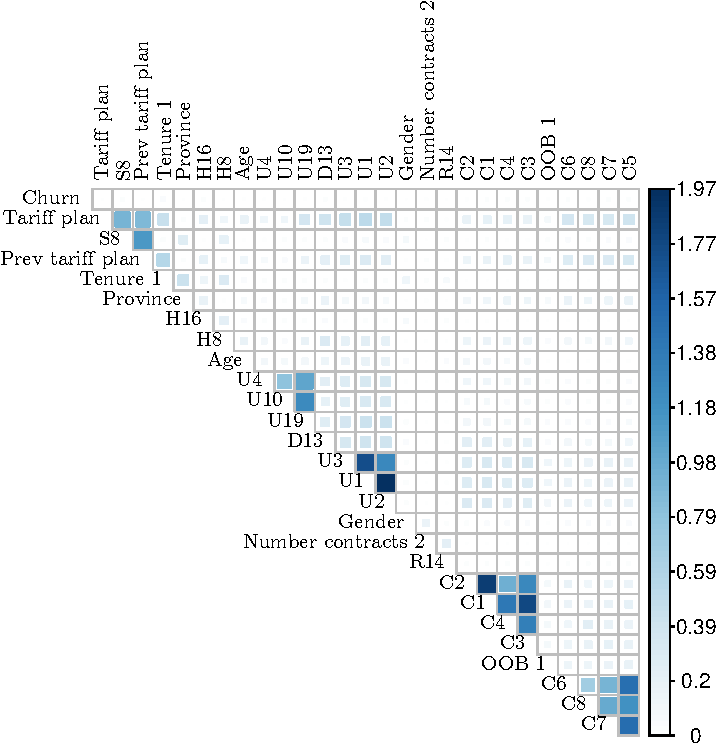
\includegraphics[width=0.8\linewidth]{figures/I_x_x.pdf}
    \caption{Mutual information matrix}
    \label{fig:I_x_x}
\end{figure}

\begin{figure}
    \centering
    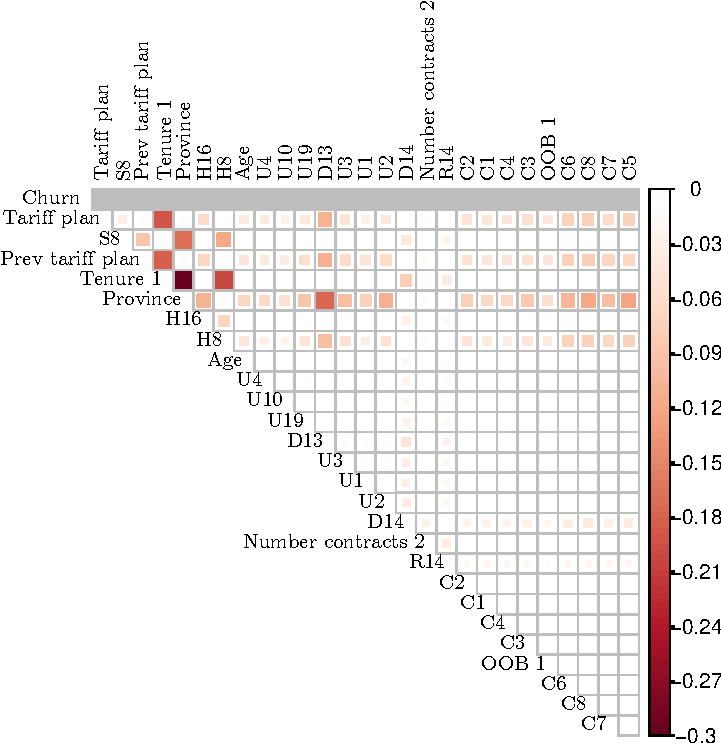
\includegraphics[width=0.8\linewidth]{figures/I_x_x_inter.pdf}
    \caption{Matrix of interaction between two variables and the churn.}
    \label{fig:I_x_x_inter}
\end{figure}

Figures \ref{fig:mimr_perso} and \ref{fig:mimr_original} show the sequence of
variables selected by the mIMR algorithm, for both our mutual information
estimator (figure \ref{fig:mimr_perso}) and the estimator assuming Gaussian
distributions (figure \ref{fig:mimr_original}). Each row corresponds to one
iteration of the algorithm. The width of the bar correspond to the value of the
mIMR criterion at this step of the algorithm, that is, the approximated value of
$I(X_k, Y) - I(\bm X_S, X_k, Y)$ where $Y$ is the churn variable, $X_k$ is the
variable under consideration and $\bm X_S$ is the set of variables selected
before $X_k$ (i.e. above $X_k$ on the plot). The two first variables have no
gain, since they are directly selected as the pair of variables having the
highest interaction with the target. Unsurprisingly, the first two variables in
figure \ref{fig:mimr_perso} are the tenure and the province (this couple of
variable has the highest negative interaction in figure \ref{fig:I_x_x_inter}).
Background knowledge, as well as figure \ref{fig:I_x_x}, indicate that the
following selected variables are not redundant with one another, up to the 9th
and 10th rows. At these rows, the two variables are both related to the data
usage. That probably indicates that the relevance term $I(X_k, Y)$ is prevailing
over the interaction term $I(\bm X_S, X_k, Y)$.

The selected variables in figure \ref{fig:mimr_original} are mostly similar to
those in \ref{fig:mimr_perso}, except that all categorical variables are not in
the first ranks. Since those are converted to as many numerical variables as
there are categorical levels, the information is spread across multiple
variables. Moreover, each of these new variables is considered to be Gaussian
distributed, therefore not allowing to estimate optimally the mutual
information. Another important difference between \ref{fig:mimr_perso} and
\ref{fig:mimr_original} is that the age and number of contracts are prevalent in
the latter. The importance of age is most probably due to the Gaussian
assumption, which is verified in this case, allowing efficient estimation of its
mutual information with other variables.

\begin{figure}
    \centering
    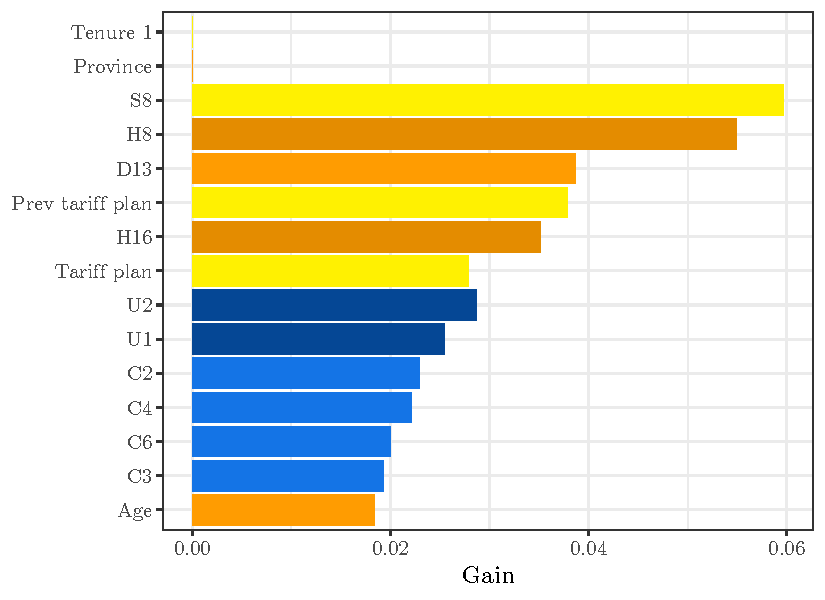
\includegraphics[width=0.9\linewidth]{figures/mimr_perso.pdf}
    \caption{Ranking of variables selected by mIMR with their respective gains,
    using the mutual information estimator of section \ref{sec:causal_intro}.
    There is no gain for the first two variables.}
    \label{fig:mimr_perso}
\end{figure}

\begin{figure}
    \centering
    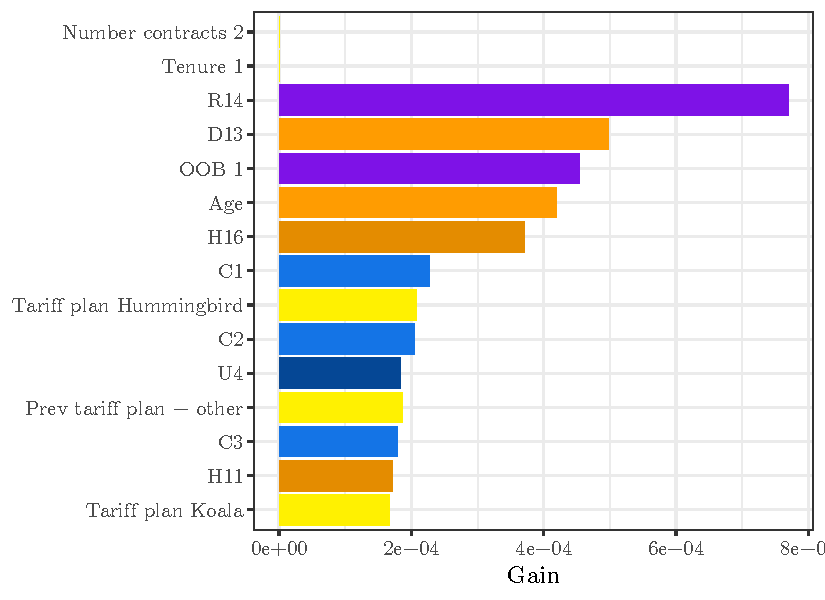
\includegraphics[width=0.9\linewidth]{figures/mimr_original.pdf}
    \caption{Ranking of variables selected by mIMR with their respective gains,
    using one-hot encoding for categorical variables and assuming Gaussian
    distributions. There is no gain for the first two variables.}
    \label{fig:mimr_original}
\end{figure}

\subsection{D2C}

The results from the D2C algorithm are shown in figure \ref{fig:d2c_proba}. To
each variable correspond a probability of being a cause of churn predicted by
the trained random forest. Since the implementation we use for D2C is designed
for numerical variables, one-hot encoding is used. All the variables present in
this plot are related to the tariff plan, previous tariff plan, province of
residence and hardware-related variables. This is consistent with results of
mIMR in figure \ref{fig:mimr_perso}, except for the second and last rows,
related to the customer gender. Mobile data usage variables are also present and
are the only variables related to service usage in this graph.

We do not believe that gender has a causal relationship with churn, and this
rank is most probably due to an artifact in the encoding of variables. Indeed,
in the data preparation process, we noticed that data entries labeled as
churners tend to have more often missing values in categorical variables. While
this issue has been resolved, an unforeseen problem may have persisted in the
gender variable.

\begin{figure}
    \centering
    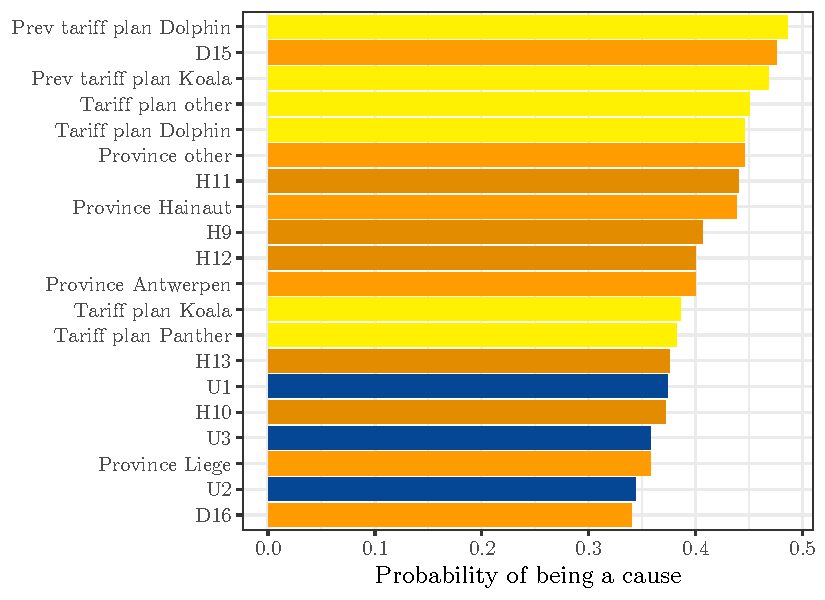
\includegraphics[width=0.9\linewidth]{figures/d2c_proba.pdf}
    \caption{Probability of causal link predicted by D2C}
    \label{fig:d2c_proba}
\end{figure}

\section{Discussion}

The output of the GS and IAMB algorithm correspond to the Markov blanket,
indistinguishably causes, effects and spouses of churn. On the other hand, mIMR
and D2C focus explicitly on direct causes, but a numerical score is provided for
each variable. A choice of threshold has to be made on which variables we
consider to be predicted as causes by these algorithms.

For the mIMR in figure \ref{fig:mimr_perso}, we include all variables up to the
9th and do not consider relevant the following ones. As discussed earlier, the
9th and 10th variables are mostly redundant with one another. Therefore, we can
assume that at this threshold, the relevance term is becoming more important
than the interaction term, and the causal property of the mIMR filter is not
maintained anymore. In the case of mIMR with Gaussian assumption, the threshold
is fixed at the 7th variable, since the following variables show a clear and
distinct decrease in gain.

As for the output of the D2C algorithm, although there seems to be a large
number of variables, most of them are different one-hot encodings of the same
original variable. The most probable causes as predicted by D2C are solely the
tariff plan, previous tariff plan, province of residence, device manufacturer
and data usage. It seems reasonable to consider these 5 variables as predicted
causes.

We summarize the results of the 5 algorithms (with the two implementations of
mIMR) in table \ref{tab:causal_summary}. For each variable, we indicate by which
algorithm this variable was output, using the thresholds discussed above. There
is no clear-cut consensus on which variables are causes. It is however
reasonable to consider the number of messages and the duration of voice calls as
\emph{not} being inferred causes of churn, since only the GS algorithm outputs
these variables. On the other hand, the tariff plan and previous tariff plan are
given by all algorithms except for PC, GS, and mIMR with Gaussian assumption. We
do not expect a categorical variable to be correctly predicted as a cause or not
using the Gaussian assumption, the theory that the tariff plan and previous
tariff plan are causes of churn are thus consistent with the observations.

\begin{table}
    \centering
    \begin{tabularx}{\textwidth}{rYYYYYY}
        \toprule
        & PC & GS & IAMB & mIMR 1 & mIMR 2 & D2C \\
        \midrule
        Tenure               & \nok & \ok  & \nok & \ok  & \ok  & \nok \\
        H14                  & \nok & \ok  & \nok & \ok  & \ok  & \nok \\
        D13                  & \nok & \ok  & \nok & \ok  & \ok  & \nok \\
        Data usage           & \nok & \ok  & \nok & \ok  & \nok & \ok  \\
        Tariff plan          & \nok & \nok & \ok  & \ok  & \nok & \ok  \\
        Prev tariff plan     & \nok & \nok & \ok  & \ok  & \nok & \ok  \\
        Out of bundle        & \nok & \ok  & \nok & \nok & \ok  & \nok \\
        Number contracts     & \nok & \ok  & \nok & \nok & \ok  & \nok \\
        S7                   & \nok & \ok  & \nok & \ok  & \nok & \nok \\
        H8                   & \nok & \nok & \nok & \ok  & \nok & \ok  \\
        Province             & \nok & \nok & \nok & \ok  & \nok & \ok  \\
        Age                  & \nok & \nok & \nok & \nok & \ok  & \nok \\
        R14                  & \nok & \nok & \nok & \nok & \ok  & \nok \\
        Messages             & \nok & \ok  & \nok & \nok & \nok & \nok \\
        Voice calls          & \nok & \ok  & \nok & \nok & \nok & \nok \\
        \bottomrule
    \end{tabularx}
    \caption{Summary of the results of causal analysis.}
    \label{tab:causal_summary}
\end{table}

In the absence of a formal procedure to assess these results, we could we will
summarize the results of causal inference from observational data to the
following statements:

\begin{itemize}
    \item The  messages, the voice calls, as well as all variables not
    represented in table \ref{tab:causal_summary}, are considered as most
    probably \emph{not inferred causes of churn}.
    \item The tariff plan and previous tariff plan are considered as most
    probably \emph{inferred causes of churn}.
    \item The inferred causal relationship of other variables in the table
    \ref{tab:causal_summary} is undecided.
\end{itemize}

In the light of our prior knowledge on the causes of churn exposed in section
\ref{sec:causal_prior}, we would expect the out of bundle variable to stand out
more explicitly, but it is only given by mIMR with Gaussian assumption. However,
recall that the distribution of the out of bundle can roughly be modeled as the
exponential of a Gaussian (see figure \ref{fig:oob}). It is thus easy to
understand why the other inference methods fail to report the causal link to the
churn expected by our priors, due to the different estimators of mutual
information. If it is true that the bill shock is a true cause of churn, then
the results we observe on table \ref{tab:causal_summary} are not extraordinary.
In other words, the credence in this theory is slightly, but not significantly,
undermined.

Two of the other causes of churn according to our prior knowledge are customer
satisfaction and churn due to a move. As explained in section
\ref{sec:causal_prior}, none of the measured variables are direct proxies for
these two putative explanations of churn. The interaction of variables present
in table \ref{tab:causal_summary} might be the most direct display of the
missing causal proxies. This would also explain the presence of variables
seemingly unrelated to our prior knowledge. However, this hypothesis is somewhat
far-fetched, and conforming to the faithfulness assumption by engineering
relevant variables would be much more precise and productive.

The last of the four expected causes of churn correspond to a wrong positioning
of the customer's tariff plan. This cause is supported by the results in a more
obvious way. The tariff plan and previous tariff plan are reported as causes of
churn by D2C and mIMR, and is also considered part of the Markov blanket by
IAMB. This indicates that the wrong positioning theory is not unlikely.
